\documentclass{my_bthesis}

% 論文タイトル（日本語）
\title{個人の移動履歴の説明文生成に\\アキネーターによる再識別評価指標の提案}
% 論文タイトル（英語）
\etitle{Proposal of Re-identification Evaluation Metrics using Akinator\\for Description Generation of Personal Mobility History}

\author{文大 太郎}
\date{2025年2月8日}

\begin{document}
\maketitle

% --- 1. 要旨（大学様式：ページ番号なし） ---
\startabstractpage
\pagenumbering{gobble} 

% --- 和文要旨 ---
\begin{center}
  {\Large \textbf{要 \quad 旨}} % 文字間隔を空けて中央揃え
\end{center}

%（和文800字程度をここに記入。数式は使わない。）
IoTの近年の進歩により、センサーベースの時系列データの大規模収集が可能となったが、その複雑さゆえに分析結果を非専門家が解釈するのは困難である。このため、複雑な出力を自然言語に変換する技術への需要が高まり、大規模言語モデル（LLM）が有望な解決策として台頭している。しかし、LLMが生成するテキストは解釈可能性を向上させる一方で、新たなプライバシー上の懸念を引き起こす。

既存の研究は、生データ（例：匿名化、差分プライバシー）またはLLM推論プロセス（例：プロンプトレベルの安全対策）の保護に焦点を当ててきた生成されたテキスト自体に内在するプライバシーリスクを直接評価してはいない。このギャップを解消するため、我々はアキネーターゲームに着想を得た匿名性指標N(D)を導入する。この指標は、与えられた記述から個人を一意に特定するために必要な最小質問数を定量化する。
移動データを入力としてLLMに与え、テキスト要約を生成した後、差分プライバシー（DP）を適用し、異なるプライバシーレベル下での出力を比較した。DPはN(D)を大幅に増加させ、個人を再識別するためにより多くの質問が必要であることを示した。さらに、N(D)はDPパラメータϵの変化に敏感に反応し、従来の構造化データ指標が見逃すプライバシー変動を捉えた。

本研究は、LLMが生成する説明文における匿名性を定量化する枠組みを提案することで、NLPとプライバシー保護データ分析を橋渡しする。N(D)指標は自然言語出力のプライバシー保護を評価する直感的かつ体系的な手段を提供し、現実世界の応用において言語表現力とプライバシーのバランスを取る基盤となる。

\vspace*{1mm}
\begin{center}
\noindent \textbf{キーワード} \underline{移動履歴, LLM, 再識別, アキネーター}
\end{center}
\vspace{0.5em} % 和文と英文の間の余白

% --- 英文 Abstract ---
\begin{center}
  {\Large \textbf{Abstract}}
\end{center}
%\vspace{1em}

%（英文300語程度をここに記入。）

Recent advances in IoT have enabled large-scale collection of sensor-based time-series data, but their complexity makes analytical results difficult for non-experts to interpret. This has increased demand for methods that translate complex outputs into natural language, with large language models (LLMs) emerging as a promising solution. However, while LLM-generated text improves interpretability, it also introduces new privacy concerns.
Prior research has mainly focused on protecting either raw data, through techniques such as anonymization and Differential Privacy (DP), or the LLM inference process itself. In contrast, the privacy risk inherent in the generated natural-language output has not been directly evaluated. To address this gap, we propose a novel anonymity metric, N(D), inspired by the Akinator game, which quantifies the minimum number of questions required to uniquely identify an individual from a given description. Using mobility data, we generated textual summaries with an LLM and evaluated the effects of DP under different privacy settings. The results show that DP substantially increases N(D), indicating higher re-identification difficulty, and that N(D) sensitively captures variations in the DP parameter ϵ. Overall, this study bridges NLP and privacy-preserving data analysis by providing an intuitive framework for quantifying anonymity in LLM-generated text.

\vspace*{1mm}
\begin{center}
\noindent \textbf{keywords} \underline{Mobility History, LLM, Re-identification, Akinator}
\end{center}

\newpage % 要旨が終わったところで改ページ
\pagenumbering{arabic} % ここからページ番号を開始（必要に応じて）

% --- 2. 目次 ---
\pagenumbering{roman} % ローマ数字 (i, ii...) 開始
\tableofcontents      % 通常の目次
\clearpage

\listoffigures        % 図目次を追加
\clearpage

\listoftables         % 表目次を追加
\clearpage

% --- 3. 本文 ---
\startmaintext
\pagenumbering{arabic}


\chapter{はじめに}
\section{研究背景}
近年のIoTデバイスの普及とセンシング技術の発展は、交通移動データ（例：ICカードデータ）やヘルスケアデータ（例：歩数、消費カロリー）などの時系列センサーデータの爆発的な蓄積をもたらしている。これらのデータは、都市計画、健康管理、行動分析など多岐にわたる分野で、データ駆動型の新たな知見と価値を生み出している。しかしながら、これらの時系列データは、その大規模性と複雑な時間的・多次元的な特徴ゆえに、データ分析の専門知識を持たない非専門家にとって、分析結果や潜在的なパターンを正確に解釈し理解することが困難であるという課題を抱えている。この課題に対処するため、複雑なデータ分析の結果やパターンを人間が直感的に理解できる自然言語のテキスト記述として自動生成する技術への需要が急速に高まっている。特に、大規模言語モデル（LLM）は、複雑な情報から自然言語で要約・説明する能力が飛躍的に向上おり、この課題解決の鍵として注目されている。\cite{10.1007/11787006_1}

\section{関連研究}
このように、時系列データから自然言語の説明文を生成する技術が進展する一方で、生成されたテキスト記述に含まれるプライバシーリスクに対する懸念も同時に深刻化している。交通移動データのように個人を特定しうる詳細な情報を含むデータが、LLMを介して自然言語化されると、その再識別（Re-identification）リスクは高まる可能性がある。既存のプライバシー保護に関する研究は、主に以下の二つの側面で進展が見られる。一つ目は、生データの保護である。これは、差分プライバシー (Differential Privacy: DP) などのメカニズムを適用し、交通系ICカードデータなどの入力データ自体の匿名性を確保するアプローチである。二つ目は、LLM推論プロセスの保護である。これは、プロンプトエンジニアリングやFederated Learning (FL) の適用により、LLMへの入力プロンプトやモデルパラメータのプライバシーを保護するアプローチである。しかしながら、生成された自然言語記述の安全性を評価・運用する上では、依然として以下の三つの重要な課題が残されている。第一に、入力データに施された差分プライバシー（DP）などの匿名化効果が、LLMによるテキスト生成プロセスを経た後も、最終的な出力文においてどの程度継承・維持されているのかを検証する直接的な手段が存在しないことである。第二に、従来の指標は非構造化テキストの曖昧さに弱く、攻撃に要するコストを非専門家でも直感的に理解できる客観的な数値として定量化できていないことである。第三に、生成文の「有用性（情報の詳細さ）」と「プライバシーリスク」という複雑なトレードオフを、体系的に評価・最適化するための基盤が確立されていないことである。

\section{研究の目的と意義}
本研究は、これらの課題を解決し、LLMが生成した自然言語の説明文の再識別リスクを定量的に測定するための新しい評価指標を提案する。具体的には、対話型クイズゲーム「アキネーター (Akinator)」に着想を得た新たな匿名性評価指標 N(D) を提案する。この指標は、与えられた自然言語記述から特定の個人を一意に特定するために必要となる最小限の質問数を定量化することにより、出力されたテキストの匿名性を直接測定することを可能にする。
定量的評価をするためにはDPを適用したデータで生成された説明文の N(D) 値が、DPを適用しない場合と比較して大幅に増加することを示す。これは、提案指標が、生成テキストにおける匿名性の向上、すなわち再識別に要する質問数の増加を明確に捉えていることを意味する。また、提案指標 N(D) が、DPパラメータ ϵ の変化に伴うプライバシーレベルの微細な変動を、LLM生成テキストの出力空間において明確に捉える高い感度と定量的信頼性を持つことを実証する。

\chapter{提案手法}
本研究は、LLMによって生成された自然言語の説明文におけるプライバシーリスクを、体系的に評価するためのフレームワークを提案する。本手法は、特定のドメインに依存せず、数値的な特徴量を持つあらゆる時系列データに適用可能である。まず提案手法の全体図を図2.1で示す。

\begin{figure*}[htbp]
\begin{center} %センタリングする
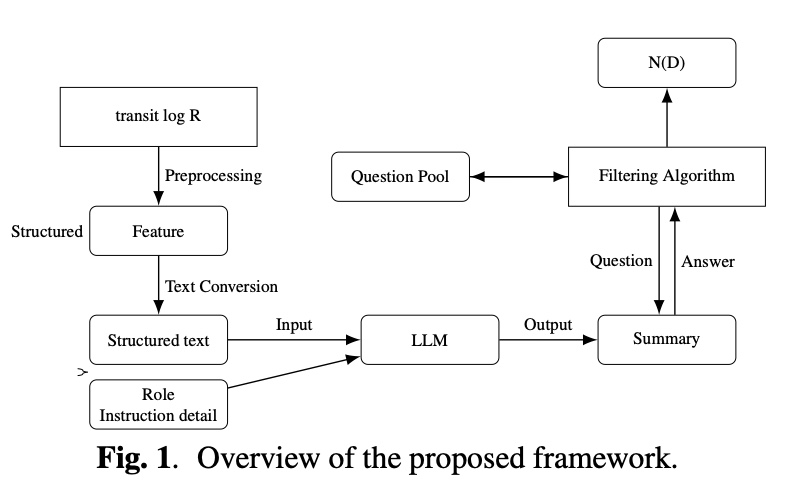
\includegraphics[width=0.75\textwidth]{./figs/framework.jpg}
\caption{Proposed Method Overview} %タイトルをつける
\label{fig:methodoverview} %ラベルをつけ図の参照を可能にする
\end{center}
\end{figure*}

\subsection{Sentiment Score for each posted data}
\label{ss:ss}

\section{概要}
提案したアルゴリズムに基づき……

\section{記述生成の形式化}


\section{匿名性指標の定義}

\section{質問選択の最適化}

\section{評価アルゴリズムの全体プロセス}





\chapter{評価}

\section{実験方法}

\subsection{実験1}

\subsection{実験2}

\section{実験結果}

\begin{table}[htbp]
\caption{Impact of Differential Privacy on Re-identification risk Depth}
\label{tbl:dp_effect}
\centering
\begin{tabular}{lrrrr}
\noalign{\hrule height 1pt}
status & mean & max & min & users \\
\noalign{\hrule height 1pt}
DP ($\epsilon=1$) & 28.2 & 50 & 14 & 10 \\
DP ($\epsilon=3$) & 24.5 & 50 & 14 & 10 \\
NO DP               &  9.1 & 15 &  4 & 10 \\
\noalign{\hrule height 1pt}
\end{tabular}
\end{table}


\chapter{考察}


\section{DP処理済みデータとLLMの相互作用生成}


\section{定量的指標としてのN(D)の検証}




\section{効用とプライバシーのトレードオフへの示唆}








\chapter{参考：クロスドメイン技術候補抽出研究の図表}
\label{ch:crossdomain}

本章では、参考として、クロスドメイン技術候補抽出に関する研究で生成された図表を示す。この研究は、特許文書から課題文脈と解決手段文脈を分離し、異分野間における技術候補を抽出する手法を提案している。

\section{候補タイプの定義と実験の位置づけ}
図 \ref{fig:solution_type_quadrant} に、課題文脈類似度と解決手段文脈類似度に基づく候補タイプの概念図を示す。この図では、実験1（近接解決策型）と実験2（異質解決策型）の位置づけが明確に示されている。

\begin{figure}[htbp]
\begin{center}
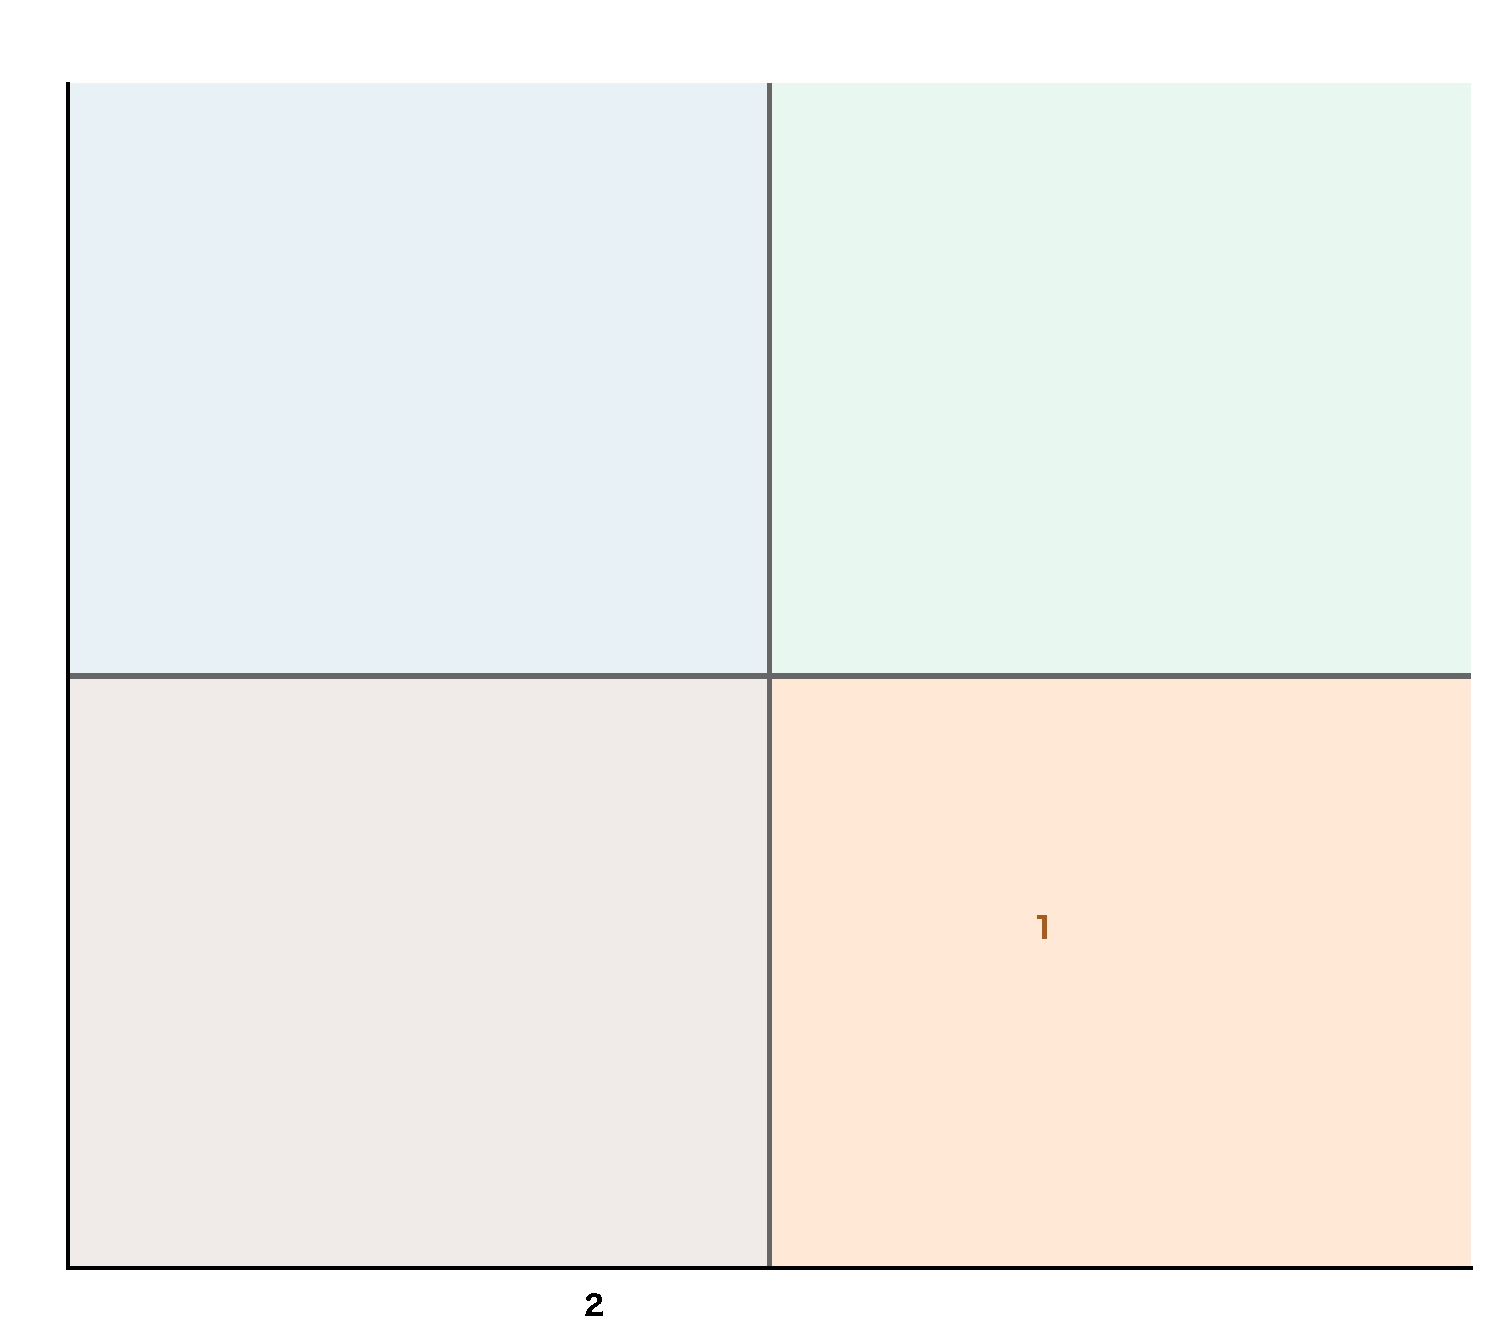
\includegraphics[width=0.85\textwidth]{./figs/solution_type_quadrant.pdf}
\caption{候補タイプと実験の位置づけ}
\label{fig:solution_type_quadrant}
\end{center}
\end{figure}

\section{提案手法の処理フロー}
図 \ref{fig:method_pipeline} に、提案手法全体の処理フローを示す。特許データから候補集合の抽出、著者確認評価に至るまでの一連のプロセスが可視化されている。

\begin{figure}[htbp]
\begin{center}
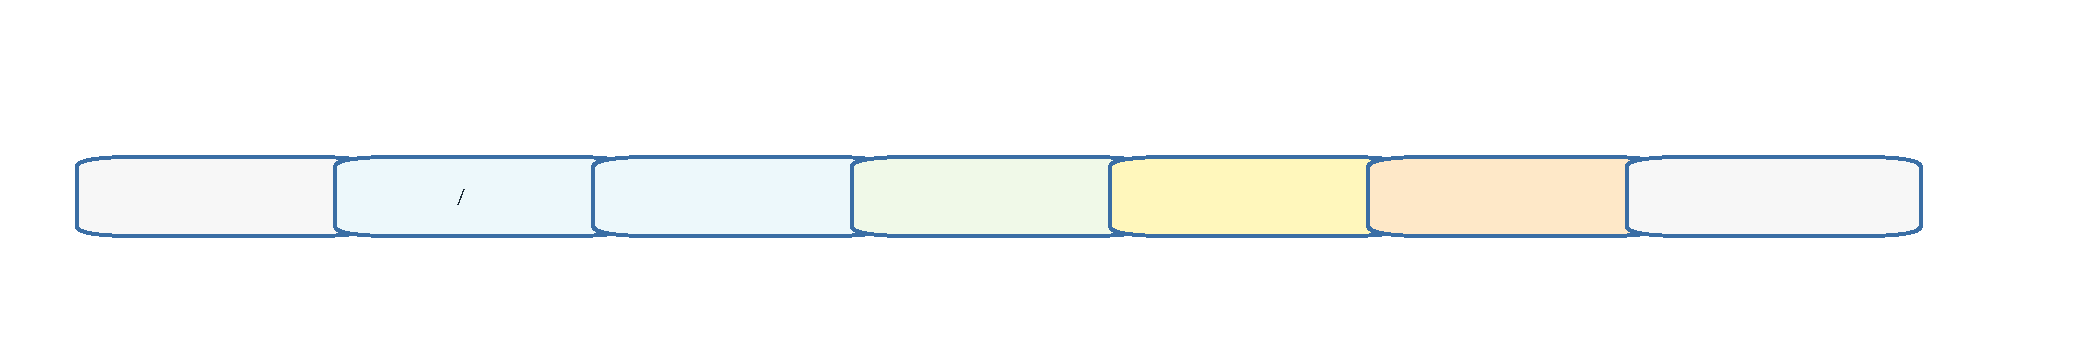
\includegraphics[width=0.95\textwidth]{./figs/method_pipeline.pdf}
\caption{提案手法の全体処理フロー}
\label{fig:method_pipeline}
\end{center}
\end{figure}

\section{実験1：U-Net候補抽出フロー}
図 \ref{fig:experiment1_pipeline} に、実験1の処理フローを示す。医療画像解析分野から製造欠陥検出分野への U-Net 関連候補抽出のプロセスが示されている。

\begin{figure}[htbp]
\begin{center}
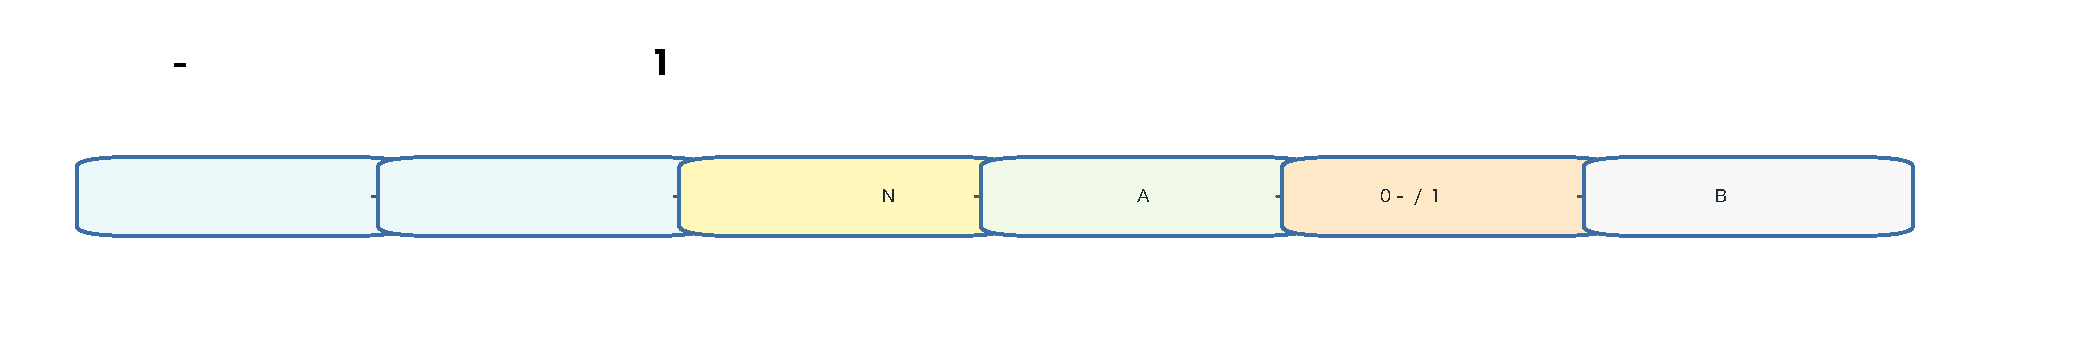
\includegraphics[width=0.95\textwidth]{./figs/experiment1_pipeline.pdf}
\caption{実験1フロー：U-Netを対象とした近接解決策型}
\label{fig:experiment1_pipeline}
\end{center}
\end{figure}

\section{実験2：異質解決策型分析フロー}
図 \ref{fig:experiment2_pipeline} に、実験2の処理フローを示す。洗浄・除去系技術を対象とした異質解決策型候補抽出のプロセスが可視化されている。

\begin{figure}[htbp]
\begin{center}
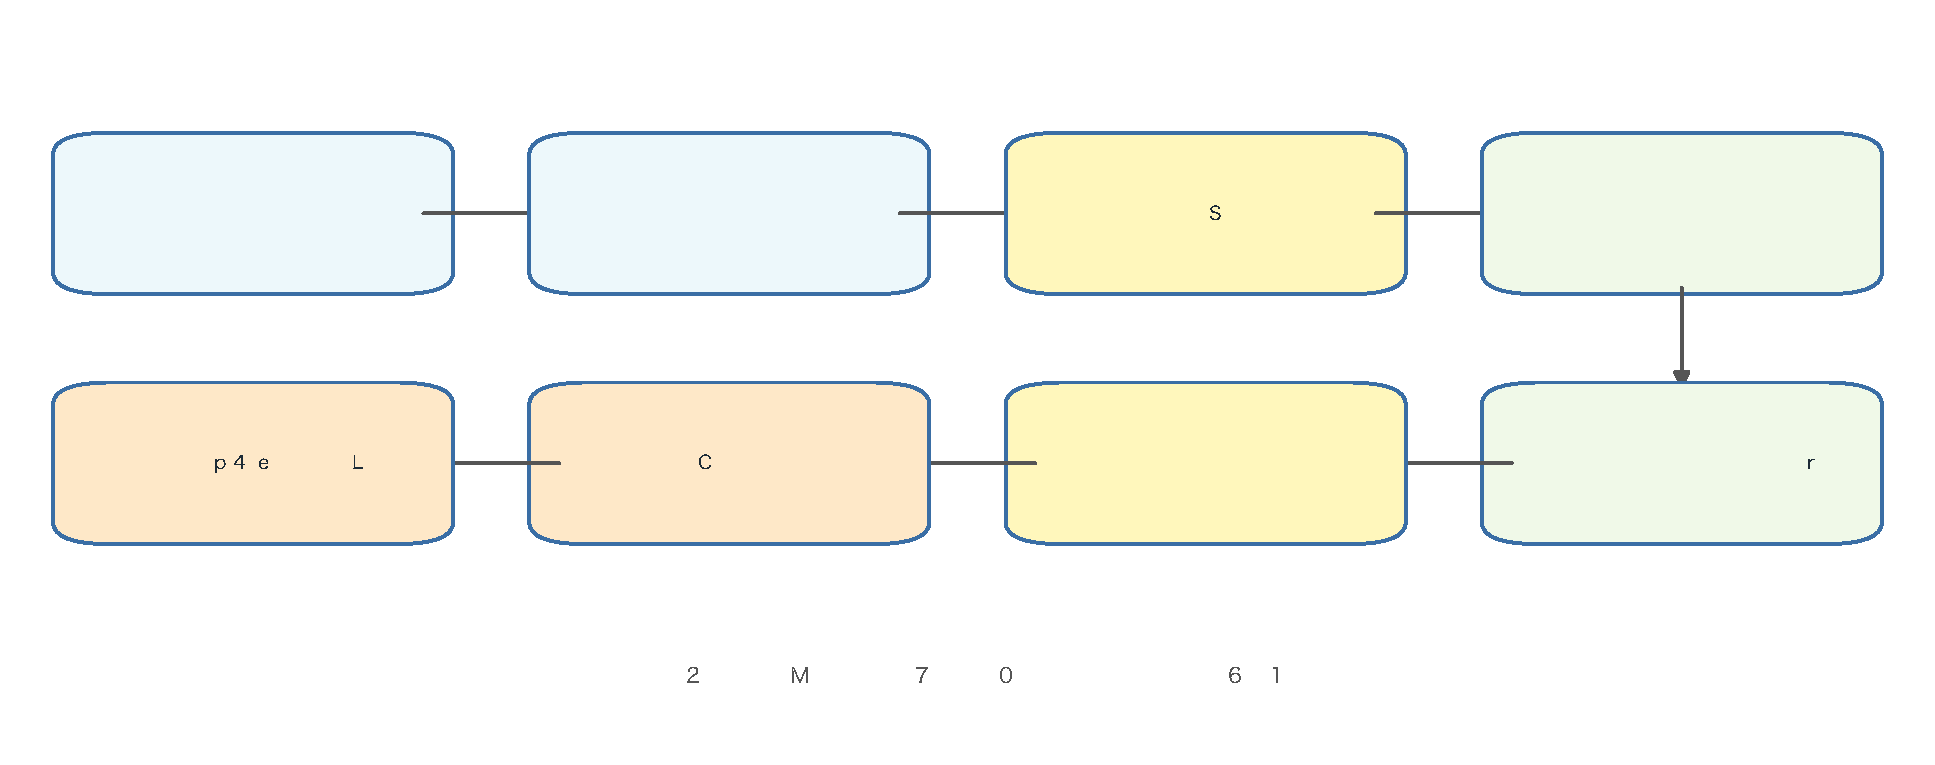
\includegraphics[width=0.95\textwidth]{./figs/experiment2_pipeline.pdf}
\caption{実験2フロー：異質解決策型の補助分析}
\label{fig:experiment2_pipeline}
\end{center}
\end{figure}

\section{実験結果}
表 \ref{tab:dataset_summary} は、実験1で使用されたデータセットのサマリーを示している。医療画像解析分野（A0）と製造欠陥検出分野（B0）におけるデータの過去・将来期間分割と U-Net の登場率が記載されている。

\begin{table}[tbp]
\centering
\small
\caption{実験1のデータセットサマリー}
\label{tab:dataset\_summary}
\begin{tabular}{llllll}
\toprule
分野 & レベル & 合計 & 過去 & 将来 & U-Net率 \\
\midrule
A0 & publication & 54100 & 10147 & 43953 & 0.030 \\
A0 & family & 30093 & 4550 & 25543 & 0.038 \\
B0 & publication & 44364 & 4307 & 40057 & 0.007 \\
B0 & family & 28450 & 2231 & 26219 & 0.008 \\
\bottomrule
\end{tabular}
\end{table}


表 \ref{tab:experiment1_results} に、実験1の著者確認評価結果を示す。提案手法による候補抽出の有効性が複数の指標で検証されている。

\begin{table}[tbp]
\centering
\small
\caption{実験1の著者確認評価サマリー}
\label{tab:experiment1\_results}
\begin{tabular}{lllll}
\toprule
グループ & 件数 & 平均スコア & 妥当性率 & 代表的フラグ \\
\midrule
baseline & 90 & 1.63 & 0.533 & 34 \\
baseline\_random & 10 & 2.20 & 0.800 & 6 \\
proposed & 43 & 1.53 & 0.465 & 16 \\
\bottomrule
\end{tabular}
\end{table}


表 \ref{tab:experiment1_baseline_comparison} に、提案手法と全文類似上位ベースラインの比較結果を示す。候補タイプ別の評価結果が整理されている。

\begin{table}[tbp]
\centering
\small
\caption{実験1ベースライン比較}
\label{tab:experiment1\_baseline\_comparison}
\begin{tabular}{llllllll}
\toprule
候補タイプ & 件数 & 平均スコア & 妥当性率 & 強い & 妥当 & 弱い & 不適切 \\
\midrule
frequency\_top\_baseline & 30 & 2.27 & 0.767 & 17 & 6 & 5 & 2 \\
fulltext\_low\_rank\_baseline & 10 & 2.20 & 0.800 & 4 & 4 & 2 & 0 \\
fulltext\_top\_baseline & 30 & 0.567 & 0.167 & 1 & 4 & 6 & 19 \\
future\_growth & 10 & 1.10 & 0.300 & 2 & 1 & 3 & 4 \\
proposed\_top & 23 & 1.61 & 0.522 & 5 & 7 & 8 & 3 \\
true\_random\_baseline & 30 & 2.07 & 0.667 & 16 & 4 & 6 & 4 \\
unet\_related & 10 & 1.80 & 0.500 & 4 & 1 & 4 & 1 \\
\bottomrule
\end{tabular}
\end{table}


表 \ref{tab:experiment2_label_summary} に、実験2の評価ラベル分布を示す。異質解決策型における候補の解釈可能性が確認されている。

\begin{table}[tbp]
\centering
\small
\caption{実験2評価ラベルサマリー}
\label{tab:experiment2\_label\_summary}
\begin{tabular}{ll}
\toprule
ラベル & 件数 \\
\midrule
◎ 強い候補 & 11 \\
○ 妥当候補 & 5 \\
△ 弱い候補 & 12 \\
× 不適切候補 & 18 \\
\bottomrule
\end{tabular}
\end{table}


表 \ref{tab:experiment2_cluster_summary} に、実験2のクラスタレベル評価結果を示す。各クラスタにおける候補品質が分析されている。

\begin{table}[tbp]
\centering
\small
\caption{実験2クラスタレベルの評価サマリー}
\label{tab:experiment2\_cluster\_summary}
\begin{tabular}{llllllll}
\toprule
クラスタ & 件数 & 強い & 妥当 & 弱い & 不適切 & 強い/妥当率 & 広い候補率 \\
\midrule
adhesive\_cleaning & 7 & 2 & 0 & 0 & 5 & 0.286 & 0.286 \\
circuit\_board\_cleaning & 3 & 1 & 1 & 1 & 0 & 0.667 & 1.000 \\
cmp\_polishing\_post\_cleaning & 12 & 0 & 0 & 5 & 7 & 0.000 & 0.417 \\
flux\_electronic\_component\_cleaning & 5 & 1 & 1 & 2 & 1 & 0.400 & 0.800 \\
photoresist\_resin\_mask\_removal & 6 & 2 & 0 & 2 & 2 & 0.333 & 0.667 \\
semiconductor\_substrate\_cleaning & 6 & 5 & 1 & 0 & 0 & 1.000 & 1.000 \\
silicon\_wafer\_cleaning & 7 & 0 & 2 & 2 & 3 & 0.286 & 0.571 \\
\bottomrule
\end{tabular}
\end{table}


表 \ref{tab:experiment_comparison} に、実験1と実験2の評価結果の比較を示す。主分析と補助分析の性質の違いが明確に表れている。

\begin{table}[tbp]
\centering
\small
\caption{実験1と実験2の評価結果比較}
\label{tab:experiment\_comparison}
\begin{tabular}{lllll}
\toprule
実験 & 評価ユニット数 & 平均スコア & 妥当件数 & 妥当性率 \\
\midrule
実験1 & 143 & 1.64 & 76 & 0.531 \\
実験2 & 46 & 1.20 & 16 & 0.348 \\
\bottomrule
\end{tabular}
\end{table}



\chapter{おわりに}
%ここのチャプターで結論と今後の展望



% --- 4. 謝辞 ---
\chapter*{謝辞}
本研究は、JSPS科研費（24K05080）および大分大学研究力強化促進事業（BURST）の助成を受けたものです。

% --- 5. 業績 ---
%ここに研究業績を追加していく

\chapter*{業績}
\addcontentsline{toc}{chapter}{業績}

\section*{国内学会}

\begin{enumerate}[label={[\arabic*]}, leftmargin=3.5em, labelsep=1em, itemsep=1.5ex]
    % --- 業績 1 ---
    \item \textbf{甲斐 歩夢}, 大知 正直
    \par \textit{「個人の移動履歴の説明文生成におけるアキネーターによる再識別評価指標の提案」}
    \par 2025年度電気・情報関係学会九州支部連合大会（第78回連合大会）講演論文集, 06-2P-12, 2025年9月.（査読なし）

    % --- 今後増える場合はここに追加 ---
\end{enumerate}

\section*{国際学会}

\begin{enumerate}[label={[\arabic*]}, leftmargin=3.5em, labelsep=1em, itemsep=1.5ex]
    % --- 業績 1 ---
    \item \textbf{Ayumu Kai}, Ochi Masanao
    \par \textit{「Anonymity Evaluation  Algorithm for Generating Explanatory Texts Targeting Individual Movement Histories」}
    \par AROB（査読あり）

    % --- 今後増える場合はここに追加 ---
\end{enumerate}


% --- 6. 参考文献 ---
\bibliographystyle{ieeetr}
\bibliography{refs} % 学会で使っていた refs.bib を流用

\end{document}